\documentclass{standalone}
\usepackage{pgfplots}
\pgfplotsset{compat=1.18}

\begin{document}
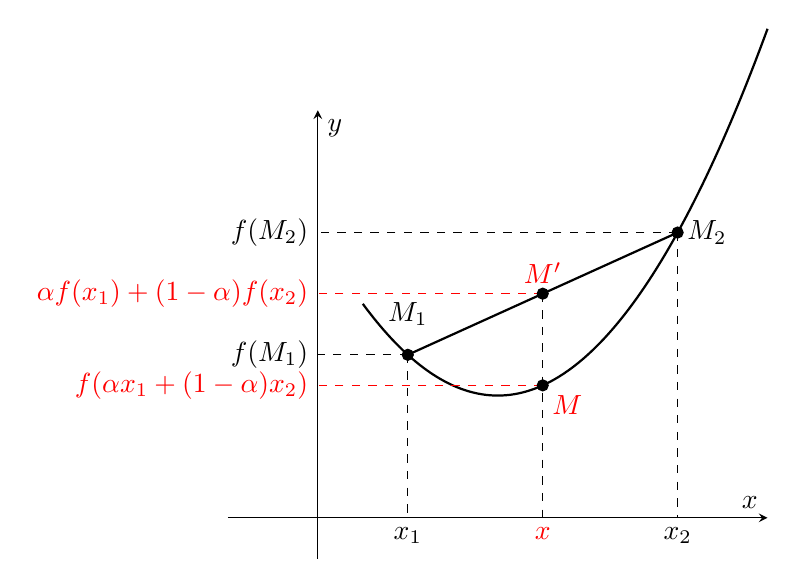
\begin{tikzpicture}
\begin{axis}[
    axis lines=middle,
    xlabel={$x$},
    ylabel={$y$},
    xmin=-1, xmax=5,
    ymin=-1, ymax=10,
    domain=0:5,
    samples=100,
    ticks=none,
    % xtick={1,2,3},
    % ytick={1,4,9},
    clip=false
]

% Plot the parabola y = x^2
\addplot [thick, black, domain=0.5:5] {(x-2)^2+3};

\addplot [only marks, mark=*] coordinates {(1,4) (4,7) (2.5,5.5) (2.5,3.25)};

% Label the points
\node [above=0.25cm] at (axis cs:1,4) {$M_1$};
\node [right] at (axis cs:4,7) {$M_2$};
\node [red, above] at (axis cs:2.5,5.5) {$M'$};
\node [red, below right] at (axis cs:2.5,3.25) {$M$};

% Draw the secant line M_1 M_2: y = x + 1
\addplot [thick, domain=1:4] {x + 3};

\draw [dashed] (1,4) -- (0,4);
\draw [dashed] (4,7) -- (0,7);
\draw [red, dashed] (2.5,5.5) -- (0,5.5);
\draw [red, dashed] (2.5,3.25) -- (0,3.25);

\draw [dashed] (1,4) -- (1,0);
\draw [dashed] (4,7) -- (4,0);
\draw [dashed] (2.5,5.5) -- (2.5,0);

\node [left] at (axis cs:0,4) {$f(M_1)$};
\node [left] at (axis cs:0,7) {$f(M_2)$};
\node [red, left] at (axis cs:0,5.5) {$\alpha f(x_1) + (1 - \alpha) f(x_2)$};
\node [red, left] at (axis cs:0,3.25) {$f(\alpha x_1 + (1 - \alpha) x_2)$};

\node [below] at (axis cs:1,0) {$x_1$};
\node [red, below] at (axis cs:2.5,0) {$x$};
\node [below] at (axis cs:4,0) {$x_2$};
\end{axis}
\end{tikzpicture}
\end{document}